\documentclass[12pt]{article}
\usepackage[english]{babel}
\usepackage[utf8x]{inputenc}
\usepackage{amsmath}
\usepackage{tikz}
\usetikzlibrary{arrows,automata}
\begin{document}

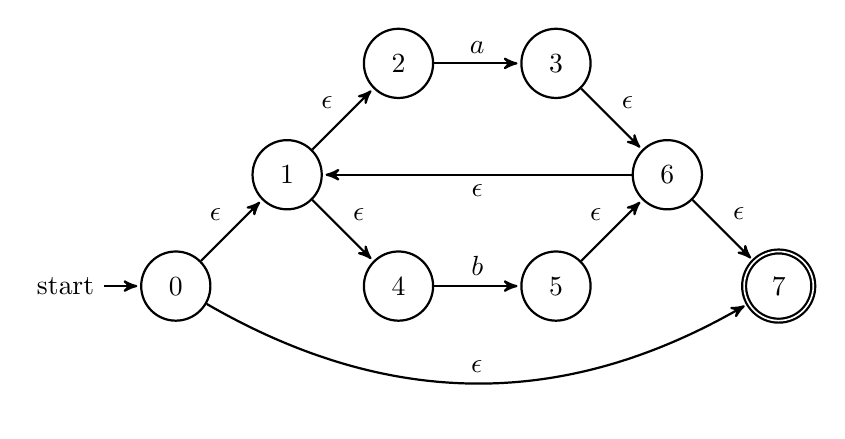
\begin{tikzpicture}[->,>=stealth',shorten >=1pt,auto,node distance=2cm,
    thick,base node/.style={circle,draw,minimum size=8pt}, real node/.style={double,circle,draw,minimum size=17pt}]

  \node[state]          (first){$1$};
  \node[state,initial]  (start) [below left of=first]{$0$};
  \node[state]          (a) [above right of=first] {$2$};
  \node[state]          (b) [right of=a] {$3$};
  \node[state]          (c) [below right of=first] {$4$};
  \node[state]          (d) [right of=c] {$5$};
  \node[state]          (e) [below right of=b] {$6$};
  \node[state,accepting]   (f)  [below right of=e] {$7$};
  
  \path (start) edge node {$\epsilon$} (first)
        (first) edge    node {$\epsilon$} (a)
        (first) edge    node {$\epsilon$} (c)
        (a) edge      node {$a$} (b)
        (b) edge       node {$\epsilon$} (e)
        (c) edge          node {$b$} (d)
        (d) edge       node {$\epsilon$} (e)
        (e) edge       node {$\epsilon$} (f)
        (e) edge       node {$\epsilon$} (first)
        (start) edge  [bend right]     node {$\epsilon$} (f)
         ;

\end{tikzpicture}
\end{document}